\chapter{Sekwencjonowanie i adnotacja genomu}
\label{section:biologiny_wstep}

\section{Sekwencjonowanie i asembling DNA}
Sekwencjonowanie to jedna z technik biologii molekularnej, pozwalająca na odczytanie kolejności nukleotydów w cząsteczce DNA.

Najlepiej byłoby, gdyby projekt genomu reprezentował kompletną sekwencję nukleotydową wszystkich chromosomów danego gatunku. 
Jednak w rzeczywistości, istnieje wiele potencjalnych problemów związanych z procesem sekwencjonowania. Nie istnieje bowiem, jedna, prawdziwa sekwencja dla gatunku z powodu indywidualnej zmienności genetycznej jednostek. 
Nawet komórki tego samego osobnika mogą różnić się w zawartości genetycznej z powodu mutacji somatycznych. Złożony genom będzie tylko jedną reprezentacją wariacji występującej u danego gatunku. 
Zasadniczo sekwencjonuje się tylko jednego osobnika, ale czasami genom stanowi konsensus wielu połączonych próbek (projekt HUGO). 
Należy zdawać sobie sprawę, że procesowi sekwencjonowania zawsze będą towarzyszyć błędy na poziomie poszczególnych nukleotydów oraz ich kolejności (błędy montażu). 
Każdy złożony genom jest wynikiem serii złożeń metodami heurystycznymi i powinien być traktowany jako robocza hipoteza.

\begin{figure}[h]
	\centering
	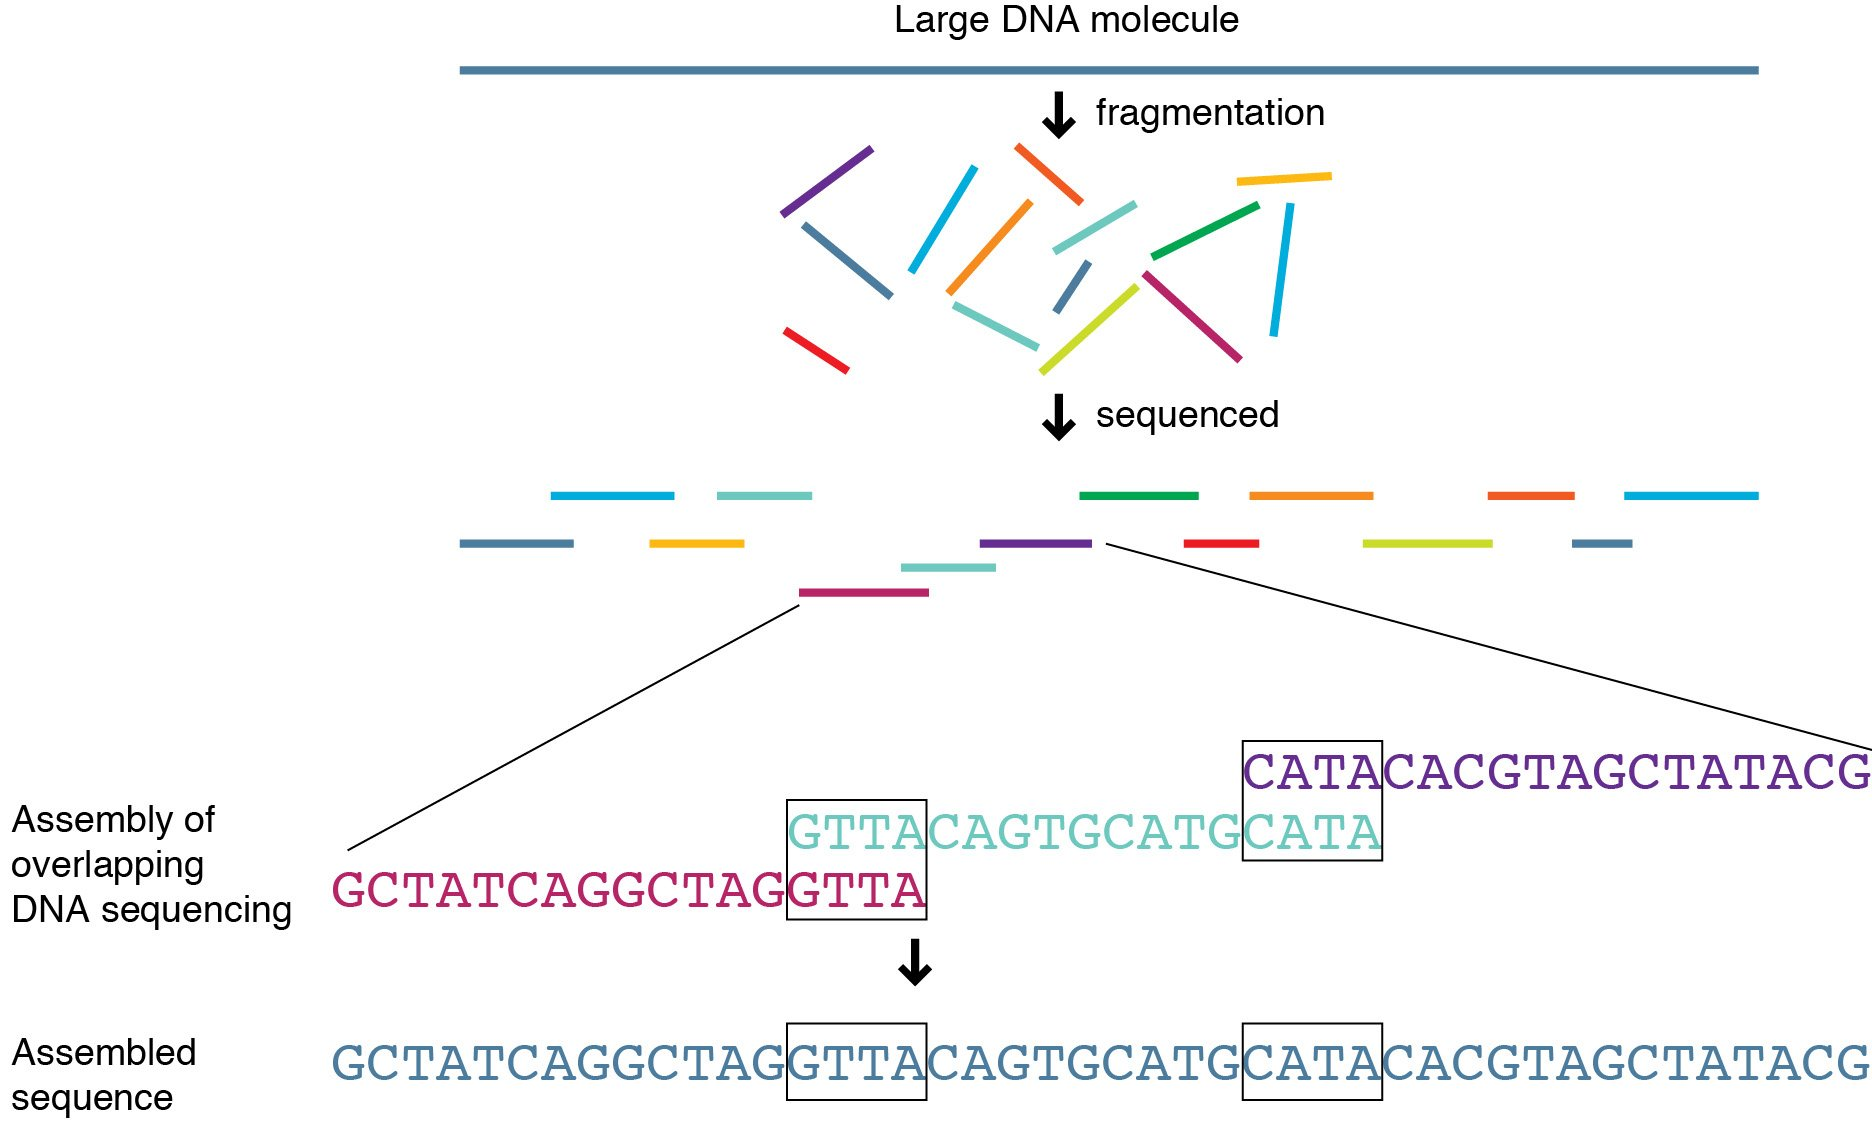
\includegraphics[width=0.9\textwidth]{img/sequenctioning-process.png}
	%zdjecie z %http://knowgenetics.org/whole-genome-sequencing/
	\caption{Schemat sekwencjonowania}
	\vspace{-0.5cm}
	\caption*{\scriptsize Źródło: \url{http://knowgenetics.org/whole-genome-sequencing/}}
	\label{img:schemat-sekwencjonowania}
\end{figure}

Większość projektów, w początkowej fazie sekwencjonowania kieruje się strategią polegającą na losowym pocięciu DNA na bardzo małe fragmenty.
W zależności od wykorzystanej technologii, fragmenty mogą mieć różne długości. Istnieje trend w kierunku przeprowadzania odczytów technikami dającymi coraz krótsze fragmenty. 
Tradycyjne sposoby (Sanger) dawały fragmenty długości około 1000 par zasad. Obecnie wykorzystywane techniki dające najkrótsze rezultaty osiągają wyniki rzędu dziesiątek pz. (SOLiD, Illumina - rys.\ref{img:sekwencjoner-illumina}).

\begin{figure}[h]
	\centering
	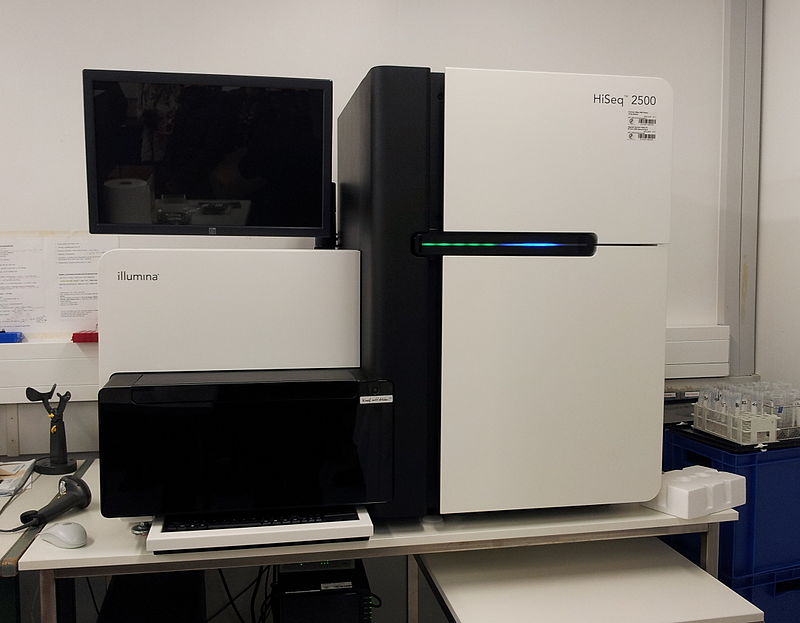
\includegraphics[width=0.75\textwidth]{img/sekwencjoner-illumina.jpg}
	%zdjecie z http://wiedza.alkahest.umcs.pl/jak-limfocyty-t-przekazuja-informacje/
	\caption{Sekwencjoner Illumina HiSeq 2500}
	\vspace{-0.5cm}
	\caption*{\scriptsize Źródło: \url{http://wiedza.alkahest.umcs.pl/jak-limfocyty-t-przekazuja-informacje/}}
	\label{img:sekwencjoner-illumina}
\end{figure}

Następie, w procesie asemblingu, fragmenty sekwencji są składane w dłuższe odcinki. Dobór algorytmu jest zależny od długości odcinków zsekwencjonowanych w poprzednim etapie. Jest to proces skomplikowany i wykorzystywane są do tego zasobożerne programy. 
Efektem początkowego składania sekwencji są kontigi.
Na dalszych etapach, po analizach wykorzystujących biblioteki dłużych sekwencji DNA, kontigi są zespalane w struktury zwane skafoldami.
Mają one zazwyczaj postać sekwencji z lukami o znanej długości - dziury oznaczane są znakiem ,,N''.

\section{Adnotacje}
Aby wykorzystać cały potencjał sekwencji genomu, musi on zostać opatrzony adnotacjami, które zawierają istotne informacje z biologicznego punktu widzenia. Kompletna adnotacja genomu stanowi duże wyzwanie dla biologów, a jej wyniki są w dużej mierze uzależnione od jakości złożenia genomu w procesie asemblingu.

Adnotacja genomu jest procesem odnalezienia regionów kodujących, zidentyfikowania genów oraz określenia funkcji jakie pełnią. Adnotacją możemy nazywać np. przypis będący notatką dodaną jako wyjaśnienie bądź komentarz. Dzielą się na przypisy:
\itemize{
	\item strukturalne (identyfikacja obiektów genomowych)
	\item funkcjonalne (biologiczne informacje związane z obiektami genomowymi)
}
\\
Proces adnotacji można podzielić na 3 główne fazy:
\enumerate{
	\item Identyfikacja niekodujących fragmentów.
	\item Przewidywanie genów.
	\item Dołączenie biologicznych informacji.
}\\

Większość technik wykorzystuje narzędzia oparte o wyszukiwanie homologicznych sekwencji używając do tego celu publiczne bazy danych genomów. Przewidywanie genów to czynność mająca na celu zidentyfikowanie fragmentów DNA, które odpowiedzialne są za kodowanie białek. Wśród organizmów zbudowanych z komórek posiadających jądro komórkowe z chromosomami (eukarioty), odcinki kodujące sekwencję aminokwasów nazywane są eksonami, które zazyczaj oddzielone są fragmentami niekodującymi - intronami (rys.\ref{img:intron-exon}).

\begin{figure}[h]
	\centering
	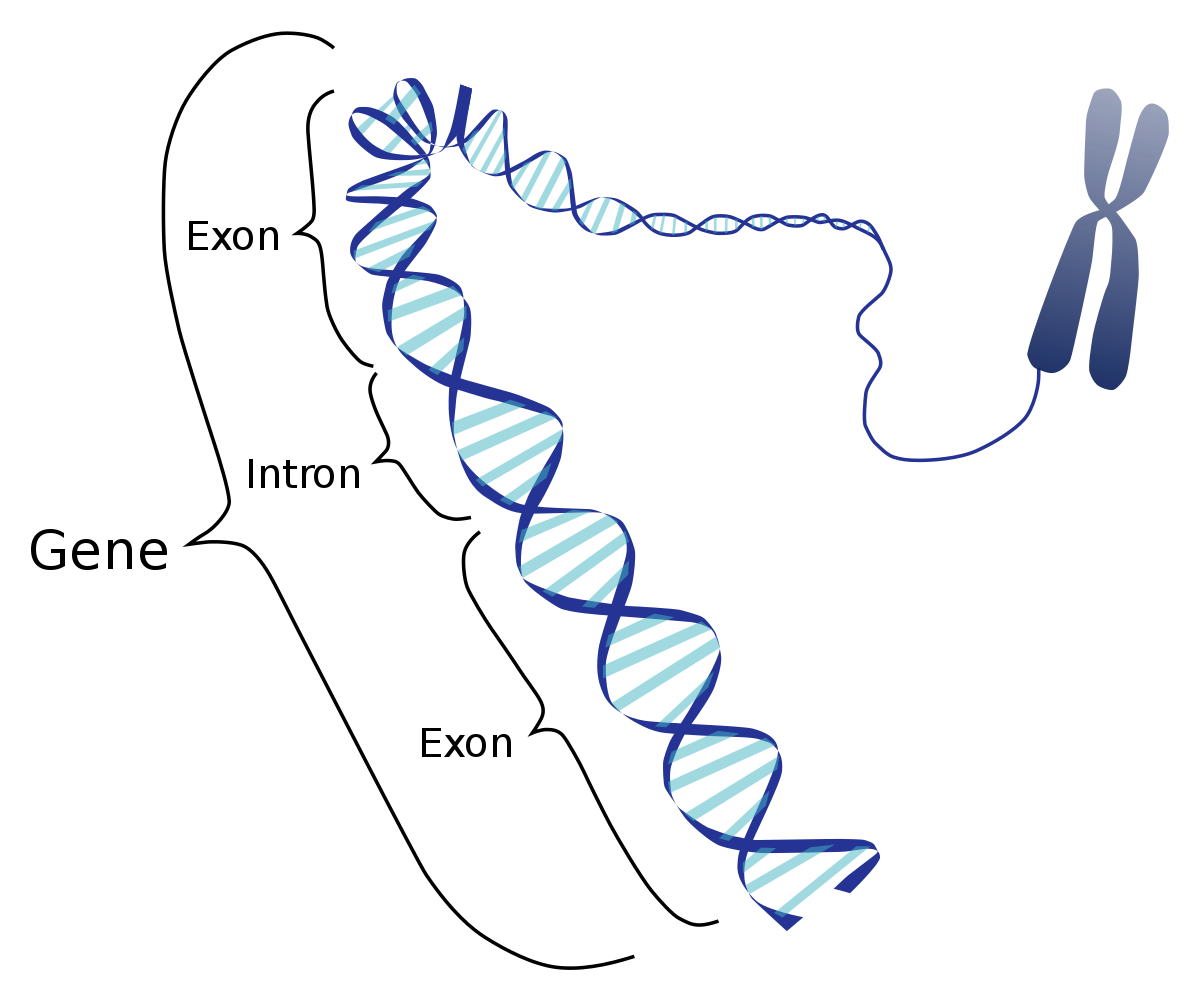
\includegraphics[width=0.75\textwidth]{img/intron-exon.png}
	\caption{Reprezentacja intronów i eksonów z genem zawierającym pojedynczy intron i dwa eksony.}
	\vspace{-0.5cm}
	\caption*{\scriptsize Źródło: \url{https://en.wikipedia.org/wiki/File:Gene\_Intron\_Exon\_nb.svg}}
	\label{img:intron-exon}
\end{figure}



\section{Prezentacja danych}

\section{Przegląd literatury}